\documentclass[final,12pt]{article}
%
\usepackage[left=1in, top=1in, bottom=1in, right=1in]{geometry}

% packages 
\usepackage{latexsym,amssymb,amsmath,color}
%\usepackage{theorem}
\usepackage{graphicx}
\usepackage[colorlinks=true]{hyperref}
\hypersetup{urlcolor=blue, citecolor=red}
%\usepackage{algorithmic}
%\usepackage{algorithm}
\usepackage{cite}
\usepackage[table]{xcolor}



% -------------- macros
\newcommand{\p}{\partial}
\def\Cb{\overline{C}}

\newcommand{\R}{\mathbb{R}}
\newcommand{\N}{\mathbb{N}}
\newcommand{\cov}{\mathrm{cov}}
\newcommand{\iid}{\stackrel{iid}{\sim}}
\newcommand{\F}{\mathcal{F}}%
\newcommand{\be}{\begin{equation}}
\newcommand{\ee}{\end{equation}}
\newcommand{\bea}{\begin{eqnarray}}
\newcommand{\eea}{\end{eqnarray}}
%\newcommand{\p}{\partial}
\newcommand{\ttt}{\tilde}
%
\def\Wb{\overline{W}}
\def\td{\tilde \delta}
\def\tL{\tilde L}
\def\tU{\tilde U}
\def\tt{\tilde t}
\def\Vector#1{\mbox{\boldmath $#1$}}
\def\vH{{\Vector H}}
\def\vx{{\Vector x}}
\def\vy{{\Vector y}}
\def\vz{{\Vector z}}
\def\vj{{\Vector j}}
\def\vk{{\Vector k}}
\def\vt{{\Vector t}}
\def\ve{{\Vector e}}
\def\vb{{\Vector b}}
\def\vg{{\Vector g}}
\def\vn{{\Vector n}}
\def\vp{{\Vector p}}
\def\vr{{\Vector r}}
\def\vS{{\Vector S}}
\def\vV{{\Vector V}}
\def\vY{{\Vector Y}}
\def\vX{{\Vector X}}
\def\vv{{\Vector v}}
\def\vu{{\Vector u}}
\def\vQ{{\Vector Q}}
\def\vZ{{\Vector Z}}
\def\vN{{\Vector N}}
\def\vF{{\Vector F}}
\def\vC{{\Vector C}}
\def\vq{{\Vector q}}
\def\vom{{\Vector \omega}}
\def\vtau{{\Vector \tau}}
\def\F{{\rm\bf F}}
\def\sech{{\rm sech}}
\def\funnyzeta{\varsigma}
\def\tQ{\stackrel{\ldots}{Q}}
%
\def\Re{{\rm Re}}
\def\Sc{{\rm Sc}}
\def\Pe{{\rm Pe}}
\def\Pr{{\rm Pr}}
\def\Da{{\rm Da}}
\def\rf{{\rm ref}}
\def\eps{{\varepsilon}}
\def\ep{\epsilon'}
\def\O{{\rm O}}
\def\1{{\rm 1}}
\def\so{^{\rm (0)}}
\def\s1{^{\rm (1)}}
\def\d{{\rm d}}
\def\ttm{^{{\rm ttm}}}
\def\img{^{\rm im}}
\def\si{^{\rm si}}
%
\def\ol{\overline}
%
\def\tn{^{n}}
\def\tnm{^{n-1}}
\def\new#1{{\bf #1}}
%\def\new#1{{#1}}

\renewcommand{\L}{\mathcal{L}}
\newcommand{\Q}{\mathcal{Q}}
\newcommand{\U}{\mathcal{U}}
\newcommand{\G}{\mathcal{N}}
\newcommand{\V}{\mathcal{V}}
\renewcommand{\P}{\mathrm{P}}
\newcommand{\B}{\mathcal{B}}
\renewcommand{\vec}[1]{{\mathchoice
                     {\mbox{\boldmath$\displaystyle{#1}$}}
                     {\mbox{\boldmath$\textstyle{#1}$}}
                     {\mbox{\boldmath$\scriptstyle{#1}$}}
                     {\mbox{\boldmath$\scriptscriptstyle{#1}$}}}}
\newcommand{\var}[1]{{\mathrm{Var}}\left( {#1} \right)}
\newcommand{\normim}[1]{\left\| {#1} \right\|_{\scriptscriptstyle L^{2}(\Omega^{*})}}
\newcommand{\avemu}[1]{\mathrm{E}\left({#1}\right)}
\newcommand{\ave}[1]{\left\langle {#1} \right\rangle}
\newcommand{\prob}[1]{\mathrm{Prob}\left\{ {#1} \right\}}
\newcommand{\ind}[1]{\mathrm{\chi}_{\scriptscriptstyle {#1} }}
\newcommand{\NISP}{\mathcal{S}}
\newcommand{\xxi}{\vec{\xi}}
\newcommand{\ip}[2]{\left( {#1}, {#2} \right)}
\newcommand{\ipmu}[2]{\left( {#1}, {#2} \right)_\mu}
\newcommand{\norm}[1]{\left\| {#1} \right\|_{\scriptscriptstyle L^{2}(\Omega)}}
\newcommand{\normone}[1]{\left\| {#1} \right\|_{\scriptscriptstyle 1}}
\newcommand{\pard}[2]{\frac{\partial{#1}}{\partial{#2}}}
%
%\newcommand{\be}{\begin{equation}}
%\newcommand{\ee}{\end{equation}}
%\newcommand{\bea}{\begin{eqnarray}}
%\newcommand{\eea}{\end{eqnarray}}
%\newcommand{\p}{\partial}
%\newcommand{\ttt}{\tilde}
%
\def\Wb{\overline{W}}
\def\td{\tilde \delta}
\def\tL{\tilde L}
\def\tU{\tilde U}
\def\tt{\tilde t}
\def\Vector#1{\mbox{\boldmath $#1$}}
\def\vH{{\Vector H}}
\def\vx{{\Vector x}}
\def\vy{{\Vector y}}
\def\vz{{\Vector z}}
\def\vj{{\Vector j}}
\def\vk{{\Vector k}}
\def\vt{{\Vector t}}
\def\ve{{\Vector e}}
\def\vb{{\Vector b}}
\def\vg{{\Vector g}}
\def\vn{{\Vector n}}
\def\vp{{\Vector p}}
\def\vr{{\Vector r}}
\def\vS{{\Vector S}}
\def\vV{{\Vector V}}
\def\vY{{\Vector Y}}
\def\vX{{\Vector X}}
\def\vv{{\Vector v}}
\def\vu{{\Vector u}}
\def\vQ{{\Vector Q}}
\def\vZ{{\Vector Z}}
\def\vN{{\Vector N}}
\def\vF{{\Vector F}}
\def\vC{{\Vector C}}
\def\vq{{\Vector q}}
\def\vom{{\Vector \omega}}
\def\vtau{{\Vector \tau}}
\def\F{{\rm\bf F}}
\def\sech{{\rm sech}}
\def\funnyzeta{\varsigma}
\def\tQ{\stackrel{\ldots}{Q}}
%
\def\Re{{\rm Re}}
\def\Sc{{\rm Sc}}
\def\Pe{{\rm Pe}}
\def\Pr{{\rm Pr}}
\def\Da{{\rm Da}}
\def\rf{{\rm ref}}
\def\eps{{\varepsilon}}
\def\ep{\epsilon'}
\def\O{{\rm O}}
\def\1{{\rm 1}}
\def\so{^{\rm (0)}}
\def\s1{^{\rm (1)}}
\def\d{{\rm d}}
\def\ttm{^{{\rm ttm}}}
\def\img{^{\rm im}}
\def\si{^{\rm si}}
%
\def\ol{\overline}
%
\def\tn{^{n}}
\def\tnm{^{n-1}}
\def\new#1{{\bf #1}}
\newcommand{\todo}[1]{\scshape\color{red}{#1}}
%
 \def\ol{\overline}
 \def\no{\noindent}
 \def\qd{\dot{Q}}

% macros added by Alen
\newcommand{\Np}{{N_\text{p}}}
\newcommand{\Npc}{{N_\text{PC}}}
\newcommand{\alennote}[1]{{\color{blue}Alen: {#1}}}
\newcommand{\manavnote}[1]{{\color{blue}Manav: {#1}}}

\def\longrightharpoonup{\relbar\joinrel\rightharpoonup}
\def\longleftharpoondown{\leftharpoondown\joinrel\relbar}
\def\longrightleftharpoons{
  \mathop{
    \vcenter{
      \hbox{
      \ooalign{
        \raise1pt\hbox{$\longrightharpoonup\joinrel$}\crcr
          \lower1pt\hbox{$\longleftharpoondown\joinrel$}
          }
      }
    }
  }
}


\newcommand{\GG}{G}
% ----------------- end macros

\usepackage[table]{xcolor}
\usepackage{booktabs} 
\usepackage{relsize}
\usepackage{bm}
\usepackage{mathrsfs}
\usepackage{amsmath,amssymb}
\def\ol{\overline}
\def\no{\noindent}
\def\qd{\dot{Q}}
%%%%%%%FLOW DIAGRAM%%%%%%%%%%
\usepackage[latin1]{inputenc}
\usepackage{tikz}
%\usepackage[table]{xcolor}
\usetikzlibrary{positioning,shapes,arrows,arrows.meta}
\usetikzlibrary{shapes.geometric}
% Define block styles
\tikzstyle{decision} = [diamond, minimum width=2.5cm, minimum height=1cm, text centered, draw=black]
\tikzstyle{startstop} = [rectangle, draw, 
   text width=4.5em, text centered, rounded corners]
 \tikzstyle{process} = [rectangle, draw, 
   text width=9.0em, text centered]  
\tikzstyle{line} = [draw, -latex']
\tikzstyle{cloud} = [draw, ellipse, node distance=3cm,
   minimum height=2em]
   \tikzstyle{io} = [trapezium, trapezium left angle=70, trapezium right angle=110, minimum width=2cm, text width=9.5em,minimum height=1cm, text centered, draw, inner sep=0pt]
%%%%%%%%%%%%%%%%%%%%%%%%%%

\newcommand{\cs}[1]{\textcolor{blue}{CS: #1}}

%% Breakable algorithm %%%
\usepackage{algorithm,algpseudocode,float}
\usepackage{lipsum}
\makeatletter

\newenvironment{breakablealgorithm}
  {% \begin{breakablealgorithm}
   \begin{center}
     \refstepcounter{algorithm}% New algorithm
     \hrule height.8pt depth0pt \kern2pt% \@fs@pre for \@fs@ruled
     \renewcommand{\caption}[2][\relax]{% Make a new \caption
       {\raggedright\textbf{\ALG@name~\thealgorithm} ##2\par}%
       \ifx\relax##1\relax % #1 is \relax
         \addcontentsline{loa}{algorithm}{\protect\numberline{\thealgorithm}##2}%
       \else % #1 is not \relax
         \addcontentsline{loa}{algorithm}{\protect\numberline{\thealgorithm}##1}%
       \fi
       \kern2pt\hrule\kern2pt
     }
  }{% \end{breakablealgorithm}
     \kern2pt\hrule\relax% \@fs@post for \@fs@ruled
   \end{center}
  }
  \makeatother
\algdef{SE}[DOWHILE]{Do}{doWhile}{\algorithmicdo}[1]{\algorithmicwhile\ #1}%
%%%%%%%%%%%%%%%%%


%-------------------------------------------------------------------
\begin{document}

\thispagestyle{empty}
\begin{center}
\textsc{
Efficient UQ for Atomistic Simulations using Active Subspaces
}

\bigskip 
\bigskip 

Manav Vohra$^{1}$, Alen Alexanderian$^{2}$, Sankaran Mahadevan$^{1}$

\bigskip
\bigskip

\normalsize
$^1$Department of Civil and Environmental Engineering\\
Vanderbilt University\\
Nashville, TN 37235\\

\bigskip

$^2$Department of Mathematics\\
North Carolina State University\\
Raleigh, NC 27695\\

\end{center}

\vspace{6cm}

\begin{tabbing}
Corresponding Author: \hspace{5mm} \= Sankaran Mahadevan\\
       \>  Department of Civil and Environmental Engineering\\
       \>  Vanderbilt University\\
       \>  272 Jacobs Hall, VU Mailbox: PMB 351831 \\
       \>  Nashville, TN 37235 \\
       \> \\
Phone: \> (615) 322-3040 \\
Fax:   \> (615) 343-3773 \\
Email: \>  sankaran.mahadevan@vanderbilt.edu   \\
\\
Submitted to: \> \textit{Modelling and Simulation in Materials Science and Engineering} \\
\>  July 2018\\

\bigskip
\end{tabbing}

\clearpage



\baselineskip=22pt

%\tableofcontents

%\input{abstract}
%\clearpage
%
%\section{Introduction}
\label{sec:intro}

%1. Why UQ is important for this problem?
%2. Challenges pertaining to UQ. Include a table for exponential scaling. 
%3. What has been done in previous UQ studies for atomistic level simulations.
%4. How we tried to address the challenge in our previous work.
%5. How is this work different?
%6. Key contributions.
%7. Organization of the paper.

Non-equilibrium molecular dynamics (NEMD) simulations are commonly used to investigate
bulk thermal conductivity of non-metallic elements such as carbon, silicon, and
germanium~\cite{Dumitrica:2010}. The system is subjected to either a heat flux or a temperature
gradient by means of thermostatting. Resulting steady-state temperature gradient in the
former and heat exchange between the thermostats in the latter is recored. The thermal
conductivity at a given system size is hence estimated using Fourier's law. In the
so-called direct method~\cite{Schelling:2002,Turney:2009,Zhou:2009,Landry:2009,
McGaughey:2006,Ni:2009,Shi:2009,Wang:2009,Papanikolaou:2008},
the thermal conductivity is estimated at multiple values of the
system size. The inverse of thermal conductivity ($\kappa^{-1}$) is plotted against the inverse of 
system size ($L^{-1}$) and a linear extrapolation procedure is used to estimate the y-intercept
of the plot. Inverse of the y-intercept is regarded as the bulk thermal conductivity
of the system since it corresponds to an infinitely large system (in theory). 

Although widely used, severe limitations are associated with the direct method.
The validity of the linear extrapolation procedure is not well established. Recent
investigations have revealed the existence of a non-linear trend in the $\kappa^{-1}$-$L^{-1}$
relationship especially at large values of $L$~\cite{Sellan:2010} for Si. Additionally, 
thermal conductivity estimate for a given size depends upon the choice of a potential
function and associated values of its parameters. Specifically for Si, the Stillinger-Weber (SW)
inter-atomic potential is commonly used for a wide variety of applications:
%
\be
\Phi = \sum\limits_{i,j(i<j)}\phi_2(A,B,p,q,\alpha)\hspace{1mm}+\sum\limits_{i,j,k(i<j<k)}\phi_3(\lambda,\gamma)
\ee
%
However, according
to the methodology presented by Stillinger and Weber in~\cite{Stillinger:1985},
the following shortcomings must be noted:
%
\begin{itemize}
\item The SW potential function accounts for the second-order ($\phi_2$) and
third-order ($\phi_3$) atomic 
interactions. However, this representation can be inadequate in situations where 
higher order interactions become significant.  
\item Nominal values of the SW potential parameters were estimated using a 
limited search in a 7-dimensional parameter space. Regression-based parameter
estimates relied on the available set of experimental data while ensuring structural
stability. Hence, the estimates are tightly coupled with the set of data used for
calibration, and did not account for the presence of measurement uncertainty. 
\item Noise inherent in MD predictions can also be significant and
was not accounted for in the analysis. 
\end{itemize}
%
Hence, using the same set of nominal values for a wide range of Si-based systems and
applications is not ideal. It is therefore important to attribute uncertainty to the values and
investigate its impact on NEMD predictions. 

This paper aims to present a computational framework aimed at dimension reduction
for enabling the propagation of uncertainty from the SW potential parameters to the
quantity of interest (QoI) i.e. the thermal conductivity of a Si bar in an efficient manner. The
motivation for input-space dimension reduction stems from exponential scaling in
computational effort with the number of parameters, illustrated using the following
table:
%
\newcommand{\ra}[1]{\renewcommand{\arraystretch}{#1}}
\begin{table}[htbp]
\centering
\ra{1.3}
\begin{tabular}{@{}ccc@{}}\toprule
Parameters & Model Runs & Time (1h/run)\\
\bottomrule
1 & 10 & 10 hours \\
2 & 10$^2$ & 4.2 days \\
3 & 10$^3$ & 1.4 months \\
4 & 10$^4$ & 1.2 years \\
5 & 10$^5$ & 11.6 years \\
6 & 10$^6$ & 115.7 years \\
7 & 10$^7$ & 1157.41 years \\
\bottomrule
\end{tabular}
\caption{Exponential scaling of computational effort with the number of uncertain parameters.}
\end{table}
%
In the above table, we consider that in order to perform UQ, an average of 10 runs along each input dimension
is needed, and each run takes approximately an hour. We can easily compute that the time required to 
perform the analysis in a 7-dimensional input space is in the $\mathcal{O}(10^3)$ years which makes it
intractable. Note that the considered compute times do not account for simulation queue times that 
increases the time required for a run. 
Although computational gains can be realized using parallel computations and sparse grids
for efficient surrogate construction~\cite{Ma:2009,Constantine:2012,Petvipusit:2014,Vohra:2014}, 
the issue of exponential scaling would persist.  
Hence, we aim to tackle this issue by focussing our efforts on reducing the dimensionality of the problem
which is expect to yield maximum gains. In our earlier efforts, we presented a strategy~\cite{Vohra:2018b}
for constructing a surrogate for thermal conductivity using NEMD predictions and their dependence
on the SW potential parameters in a reduced space, evaluated using the derivative-based global sensitivity measures
(DGSMs)~\cite{Vohra:2018a}. The focus was therefore on determining the relative importance of the
parameters and fixing the unimportant parameters at their nominal values. On the other hand, the
framework presented in this study aims to identify key directions in the input space along which the
QoI predominantly varies. The set of directions constitute the so-called 
\textit{active subspace}~\cite{Constantine:2015}.  

The active subspace methodology relies on estimating the partial derivative of the QoI 
with respect to each uncertain input. This requirement poses a couple of limitations on its
applicability: (1) The QoI is required to be differentiable in the considered input domain, and (2)
In most complex problems, the derivative needs to be approximated using numerical techniques
which require model evaluations and thus impose computational burden. Fortunately, in this case,
the thermal conductivity is observed to exhibit a smooth dependence on the SW parameters. 
To mitigate the challenge pertaining to derivative estimation, we exploit our recent experience
involving the application of a gradient-free approach for evaluating the active subspace in
chemical kinetics applications~\cite{Vohra:2018c}. In this approach, the gradient is estimated
using a regression-based local linear approximation of the QoI and hence does not require
model evaluations. It was shown in~\cite{Vohra:2018c} that the gradient-free approach is
remarkably accurate is estimate the mean and the mode value of the uncertain QoI. However,
it did not fully capture the sensitivity associated with all uncertain inputs. Since our focus
in this study is on uncertainty propagation from inputs to the QoI, the gradient-free approach
seems like a suitable choice considering the computational effort associated with model 
evaluation for thermal conductivity of a Si bar. In fact, our findings reveal the existence of a 
1-dimensional active subspace in this case indicating enormous scope for computational savings.
Moreover, the global sensitivity measures based
on the active subspace are found to be consistent with our earlier estimates based on DGSMs. 

The remainder of this article is organized as follows. In section~\ref{sec:bg}, we provide details
pertaining to the NEMD simulation in \ref{sub:nemd}, and brief background on active subspaces
in~\ref{sub:as}. Details pertaining to the computational methodology are
provided in section~\ref{sec:method}. Results based on the active subspace methodology
implemented including verification of the reduced-space surrogate, and sensitivity analysis
are presented in section~\ref{sec:results}. Finally, we draw useful conclusions based on this
work in section~\ref{sec:conc}.

































%\bigskip
%\bigskip
%
%
%\section{Background}
\label{sec:bg}

In this section, we provide relevant details pertaining to the NEMD simulation 
in~\ref{sub:nemd}, and key theoretical aspects of the active subspace methodology 
in~\ref{sub:as}.

\subsection{NEMD simulation}
\label{sub:nemd}

The NEMD simulations in this work were performed using the LAMMPS software~\cite{Plimpton:2007}.
Specifically, the simulations were performed for a Si bar of length, $L$, subjected to a temperature gradient, 
$\left(\frac{dT}{dz}\right)$. The temperature gradient was applied by means of Langevin thermostats located
at $L/4$ and $3L/4$. Schematic illustration of the set-up and the arrangement of atoms is provided below in 
Figure~\ref{fig:setup}.
%
\begin{figure}[htbp]
\begin{center}
\begin{tabular}{cc}
  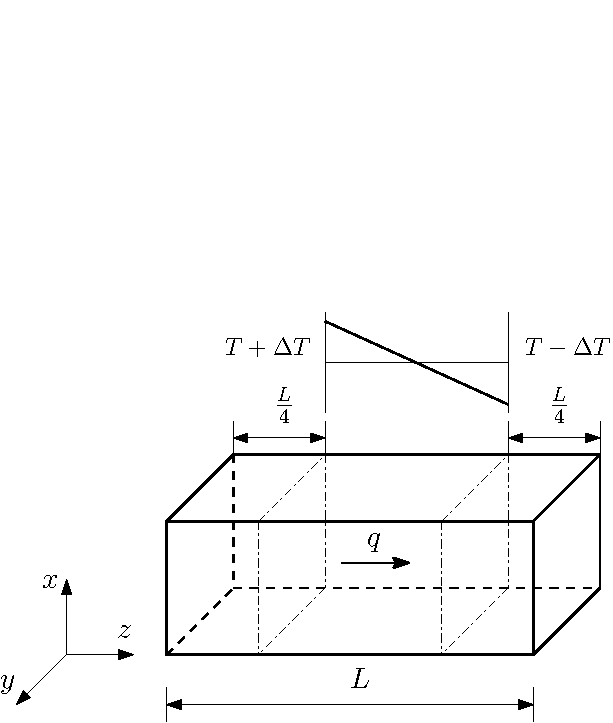
\includegraphics[width=0.48\textwidth]{./Figures/schematic}
  &
  \hspace{3mm}
  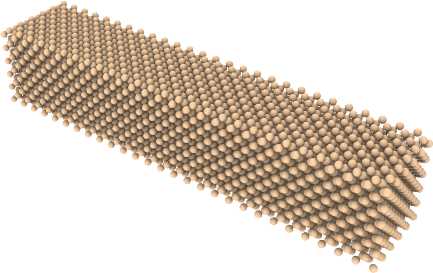
\includegraphics[width=0.40\textwidth]{./Figures/Sibar_05}
  \\ (a) & (b)
  \end{tabular}
\caption{(a) Schematic illustration of the simulation set-up for estimating the thermal conductivity of a Si bar of
length, $L$, subjected to a temperature gradient, $\left(\frac{4\Delta T}{L}\right)$, (b) 
Initial configuration of Si atoms in the bar.}
\label{fig:setup}
\end{center}
\end{figure}
%
The heat flux between the thermostats at the end of the simulation ($q$, W/m$^2$) is recorded to compute the
thermal conductivity of the Si bar using Fourier's law:
%
\be
 \kappa = \frac{q}{\left|\frac{dT}{dz}\right|} 
\ee
%
where $\left|\frac{dT}{dz}\right|$ denotes the magnitude of the applied thermal gradient. In Table~\ref{tab:input},
we provide the set of inputs used to perform the NEMD simulation. Note that the simulation run length, width, 
and height were selected to minimize temperature fluctuations during the different stages of the simulation while
ensuring a reasonable computational effort. 
%
\begin{table}[htbp]
\centering
\ra{1.3}
\begin{tabular}{@{}cc@{}}\toprule
Lattice Constant, $a$ ($\angstrom$) & 5.43 \\ 
Width, Height ($\angstrom$) & 22$a$ \\
$\Delta t$  (ps) & 0.0005 \\ 
Simulation Run Length (ps) & 320 \\ 
Boundary Condition & Periodic \\ 
Lattice Structure & Diamond \\
Inter-atomic Potential & Stillinger-Weber \\ 
\bottomrule
\end{tabular}
\caption{The set of LAMMPS inputs for performing the NEMD simulation of a Si bar illustrated in Figure~\ref{fig:setup}.}
\label{tab:input}
\end{table}
 
As illustrated in the following flow diagram, there are four stages involved in the NEMD simulation: 
NPT, NVT, NVE (I), and
NVE (II); NPT, NVT and NVE are thermodynamic ensembles used commonly in NEMD simulations. We have used
(I) and (II) here to distinguish between the two NVE ensembles. 
%
\begin{center}

NPT \hspace{5mm} $\rightarrow$ \hspace{5mm} NVT \hspace{5mm} $\rightarrow$ \hspace{5mm} NVE (I) \hspace{5mm}
$\rightarrow$ \hspace{5mm} NVE (II)
\\ \vspace{1mm}
\tiny [Relax the system]~[Equilibrate system to 300 K] \hspace{1mm} [Equilibrate thermostats] \hspace{4mm}
 [Generate Data]
\\ \vspace{1mm}

\tiny{N: Number of Atoms~~~P: Pressure~~~V: Volume~~~T: Temperature~~~E: Energy}
\end{center}
%
Initially, our NEMD simulation set-up did not comprise an NPT ensemble. However,
since computing the active subspace involves pseudorandom sampling of the marginal distributions
of the SW potential parameters, it was observed that the structural integrity of the Si bar was lost for
certain set of parameter values. To circumvent this challenge, an NPT ensemble was run
(for a sufficiently long time), prior to the NVT ensemble to ensure that the system relaxes to a 
steady value of the bar length as discussed in~\cite{Vohra:2018a}.
During the NVT stage, the system is equilibrated to a specific bulk temperature at which the thermal
conductivity of the bar is to be estimated. The NVE (I) stage involves equilibration of the thermostats
at specified temperatures. Lastly, during the NVE (II) stage, the trajectory of individual atoms during
simulation is recorded.

\subsection{Active Subspace}
\label{sub:as}

As mentioned earlier in section~\ref{sec:intro}, the active subspace is a low-dimensional space in the
input domain that sufficiently captures the variability in the QoI~\cite{Constantine:2015}.
Uncertain model inputs, $\bm{\theta}$, are parameterized as canonical random variables, 
$\bm{\xi}\in\Omega\in\mathbb{R}^{N_\theta}$, where $N_{\theta}$ denotes the number of uncertain inputs. 
Pseudorandom samples are generated according the joint probability distribution of $\xi_i$'s ($\pi_\vec\xi$).
The samples are then projected back to the physical space to evaluate the model output, $G$. The
active subspace is spanned by the dominant eigenvectors of a symmetric and positive semidefinite matrix,
$\mat{C}$:
%
\be
\mat{C} = \int_\Omega (\nabla_{\vec{\xi}}G)(\nabla_{\vec{\xi}}G)^\top dP_\vec\xi, 
\label{eq:C}
\ee
%  
where $dP_\vec\xi$ = $\pi_\vec\xi d\vec\xi$. Note that $G$ is assumed to differentiable in the considered
input domain. Additionally, $G$ and its partial derivatives in~\eqref{eq:C} are assumed to be 
L$^2$ integrable. Consider the eigenvalue decomposition of $\mat{C}$:
%
\be
\mat{C} = \mat{W}\mat{\Lambda}\mat{W}^\top.
\ee
%
where $\mat{\Lambda}$ = diag($\lambda_1,\ldots,\lambda_\Nt$) with $\lambda_i$'s sorted in
descending order:
\[
     \lambda_1 \geq \lambda_2 \geq \cdots \geq \lambda_\Nt \geq 0.
\] 
%
The matrix, $\mat{W}$ comprises orthonormal eigenvectors as its columns. The eigenpairs are partitioned
about the $p^{th}$ eigenvalue such that, \scalebox{1.25}{$\left(\frac{\lambda_p}{\lambda_{p+1}}\right)$}$\gg 1$
as follows:
%
\be
 \mat{W} = [\mat{W}_1~\mat{W}_2],~~\mat{\Lambda} = \begin{bmatrix}\mat{\Lambda}_1 & \\  &
  \mat{\Lambda}_2. 
\end{bmatrix}
\ee
%
The column space of $\mat{W}_1$ constitutes the dominant eigenspace of $\mat{C}$, regarded as the
active subspace, and $\mat{\Lambda}_1$ is the corresponding diagonal matrix with 
$\{\lambda_1,\ldots,\lambda_p\}$ as its entries. Dimension reduction is accomplished by transforming the
model output, $G(\vec\xi)$ (a function of $\Nt$ independent inputs) into $\mathcal{Y}(\vec\eta)$, a
function of $p$ independent inputs, where $\vec\eta$ = $\mat{W}_1^\top \vec\xi\in\mathbb{R}^p$, 
is referred to as the set of \textit{active variables}. Computational effort associated with UQ
is hence reduced by means of dimension reduction. However, to further decrease computational effort,
we approximate $\mathcal{Y}$ using a surrogate, $\tilde{\mathcal{Y}}$, constructed using the sequence of steps
provided in~\cite{Constantine:2015} (chapter 4), and outlined below in Algorithm~\ref{alg:surr}.
\bigskip
\begin{breakablealgorithm}
\renewcommand{\algorithmicrequire}{\textbf{Input:}}
\renewcommand{\algorithmicensure}{\textbf{Output:}}
  \caption{For constructing the surrogate model, $\tilde{\mathcal{Y}}(\mat{W}_1^\top\vec\xi)$}
  \begin{algorithmic}[1]
	\Procedure{Surrogate Model, $\tilde{\mathcal{Y}}$}{} 
	  \State Consider $N$ available data points in the full space, $(\vec\xi_i,G(\vec\xi_i))$, $i~=~1,\ldots,N$
	  \State For each $\vec\xi_i$, compute $\vec\eta_i$ = $\mat{W}_1^\top\vec\xi_i$ 
          (Note: $\mathcal{Y}(\vec{\eta}_i)$ $\approx$ $G(\vec{\xi}_i)$)
	  \State Fit a regression surface, $\tilde{\mathcal{Y}}$ to approximate $\mathcal{Y}$ using the data
                 points, $(\vec\xi_i,\mathcal{Y}(\vec\eta_i))$
	  \State Note that the overall approximation is: $G(\vec{\xi})$ $\approx$
                 $\tilde{\mathcal{Y}}(\mat{W}_1^\top\vec{\xi})$ 
	\EndProcedure
  \end{algorithmic}
  \label{alg:surr}
\end{breakablealgorithm}
\bigskip

In practice, the matrix, $\mat{C}$ is numerically approximated using model gradient estimates at random samples
in the input space as follows:
 %
 \be
 \mat{C}\approx \hat{\mat{C}} = \frac{1}{N}\sum\limits_{i=1}^{N} 
 (\nabla_{\vec{\xi}}G(\vec{\xi}_i))(\nabla_{\vec{\xi}}G(\vec{\xi}_i))^\top
 = \hat{\mat{W}}\hat{\mat{\Lambda}}\hat{\mat{W}}^\top.
\label{eq:chat}
 \ee
 %
Hence, the computational effort required for constructing $\hat{\mat{C}}$ scales with the number of samples, $N$.
To avoid excessive number of model evaluations and hence optimize the computational effort, the regression-based
approach for gradient estimation is employed to compute the active subspace
in an iterative manner as discussed in~\ref{sub:gradient} and~\ref{sub:subspace}. Furthermore, the
active subspace could be exploited to perform a global sensitivity analysis (GSA) of the SW parameters as
discussed in~\ref{sub:scores}.




































%\bigskip
%\bigskip
%
%
%\section{Proposed Methodology}
\label{sec:method}

In this section, we present the computational framework for forward and inverse UQ, based on identifying
the active subspace in NEMD simulations of bulk transport
in Si. As discussed earlier, the process involves repeated evaluations of the gradient of the model output
i.e. the bulk thermal conductivity with respect to the uncertain SW parameters at random samples
in the input domain. If a perturbation method such as finite difference is used, then gradient
estimation at $N$ samples would require $N(d+1)$ model evaluations, where $d$ is the number
of uncertain inputs. Clearly, for a large $N$, this approach would quickly become prohibitive
considering that NEMD simulations are computationally intensive. Therefore, to overcome the
computational hurdle, we rely on estimating the gradient using a regression-based approach,
whereby, a linear regression fit is performed to the available set of model evaluations. Additionally, in order
to avoid unnecessary model evaluations, the computations are performed
in an iterative manner. Specific details pertaining to gradient estimation as well as active
subspace computation are discussed further below in~\ref{sub:gradient} and~\ref{sub:subspace}. 

A surrogate model is built in the low-dimensional active subspace, which provides several benefits with respect
to the computational effort: (1) the number of atomistic simulations used to construct the surrogate are
reduced; (2) the number of samples required for forward uncertainty propagation are reduced; (3) the number samples required for GSA to assess relative contributions of the uncertain parameters to the uncertainty in
bulk thermal conductivity are reduced; and (4) the computational effort pertaining to
Bayesian calibration is reduced.
Note that (1) and (2) are discussed in~\ref{sub:surr_sub}; (3) is discussed
in~\ref{sub:scores}; and (4) is discussed in~\ref{sub:ba_method}.

\subsection{Gradient estimation}
\label{sub:gradient} 

For a given set of model evaluations at $N$ random samples in the full space input domain,
we outline the procedure for estimating the gradient of the model output, $G$, and hence the
matrix, $\hat{\mat{C}}$ in~\eqref{eq:chat}.
Note that the samples are generated
according to the joint probability distribution of the canonical random variables
($\vec\xi$), $\pi_\vec\xi$. An independent set of $M$ samples is also generated from $\pi_\vec\xi$
using Monte Carlo sampling. However, model evaluations are not required at these $M$ samples.
For each sample in $M$, a least-squares fit to $s$ nearest neighbors in
$n_0$ is performed. The value of $s$ ranges from 2 to $N-1$; $s$ = $N$ is regarded as the global approximation.
In this work, we specify $s$ as $N-1$ to capture the gradients in a leave-one-out fashion.
The slope vector ($\vec{d}_i$) of the linear regression-fit is estimated and recorded.
The collection of $\vec{d}_i$'s thus obtained are used to estimate the matrix, $\hat{\mat{C}}$. The specific 
sequence of steps is outlined in Algorithm~\ref{alg:lla}.
%
\bigskip
\begin{breakablealgorithm}
\renewcommand{\algorithmicrequire}{\textbf{Input:}}
\renewcommand{\algorithmicensure}{\textbf{Output:}}
  \caption{Constructing the matrix, $\hat{\mat{C}}$ in~\eqref{eq:chat} for a given set of $N$ model evaluations}
  \begin{algorithmic}[1]
	\Procedure{Regression-based Approach}{} 
	\State Draw $N$ random samples, $\{\bm{\xi}_j\}_{j=1}^{N}$ 
	according to $\pi_{\bm{\xi}}$.
	\State Compute $G(\bm\xi_j)$, $j=1, \ldots, N$.
	\State Draw $M$ random samples, $\{\bm{\zeta}_i\}_{i=1}^{M}$
	according to $\pi_{\bm{\xi}}$.
	\State Choose an integer $s \in [2,N-1]$ 
	\State For each $i=1, \ldots, M$, compute 
	\[
	\begin{aligned}
	\Phi_i &= \{ s \text{ nearest points in } \{\bm{\xi}_j\}_{j=1}^{N} \text{ to } \bm{\zeta}_i\}\\
	\vspace{-2mm}
	\Psi_i &= \text{subset of } G(\bm\xi_j) \text{ corresponding to the points in } \Phi_i\\
	\vspace{-2mm}
	 &{\color{white}=} \hspace{-7mm} \text{Least-squares fit:~} 
	 G(\bm\xi_j) \approx c_i + \vec{d}_i^T\bm{\xi}_j,  \bm{\xi}_j \in \Phi_i, G(\bm\xi_j) \in \Psi_i\\
	 \vspace{-2mm}
	  &{\color{white}=} \hspace{-7mm}\text{Record the slope vector,}~\vec{d}_i
	\end{aligned}
	\]
	\State Compute the matrix, $\hat{\mat{C}}$:
	\[
	\hat{\mat{C}} \approx \frac{1}{M} \sum_{i=1}^{M} \vec{d}_i\vec{d}_i^T 
	\]
	\EndProcedure
  \end{algorithmic}
  \label{alg:lla}
\end{breakablealgorithm}
\bigskip
%

\subsection{Subspace computation}
\label{sub:subspace} 

An initial set of $n_0$ samples is drawn according to the joint probability distribution
$\pi_{\vec{\xi}}$ of the inputs, $\vec{\xi}$. Model evaluations are performed at these
$n_0$ samples. 
An initial estimate of the symmetric positive semidefinite matrix, $\hat{\mat{C}}$ 
is then obtained using Algorithm~\ref{alg:lla}. The eigenvalue decomposition of 
$\hat{\mat{C}}$ is performed to obtain initial estimates of the eigenvectors and
corresponding eigenvalues:
%
\be
\hat{\mat{C}} = \frac{1}{M}\sum\limits_{i=1}^{M}\bm{d}_i\bm{d}_i^\top = \hat{\bm{W}}\hat{\bm{\Lambda}}\hat{\bm{W}}^\top.
\ee
%
At each subsequent iteration, a new set of Monte Carlo samples is generated using the joint 
probability law, $\pi_{\vec{\xi}}$. Since model evaluations are expensive, the number of new samples
is a factor of the initial number, $n_0$. The augmented set of available and newly generated model
evaluations are used to obtain improved estimates of $\hat{\mat{C}}$ using Algorithm~\ref{alg:lla}.
The eigenvalue decomposition of $\hat{\mat{C}}$ yields refined estimates of the eigenspace.
The improved eigenspace is partitioned as discussed earlier in~\ref{sub:as}
 to obtain the active subspace. For a given eigenvector ($j^{th}$) in the active subspace, 
 we compute the relative L-2 
 norm of the difference in squared values of corresponding components ($\varepsilon_j^k$) of the same eigenvector,
 computed during successive iterations (iterations $k$ and $k-1$) as follows:
%
\be
\varepsilon_j^k = \frac{\|(\hat{\mat{W}}_{1,j}^{k})^2 - 
                       (\hat{\mat{W}}_{1,j}^{k-1})^2\|_2}{\|(\hat{\mat{W}}_{1,j}^{k-1})^2\|_2}, 
                       j = 1,\ldots,p,
\label{eq:conv}
\ee
%
where $p$ denotes the dimension of the column space of $\mat{W}_1$ or the number of eigenvectors in
the active subspace.
The quantity, $\varepsilon_j^k$ is recorded as the $j^{th}$ component of $\vec\varepsilon^k$. Convergence is
established once the component with the highest magnitude is below a given tolerance, $\tau$. 
The sequence of steps for computing the active subspace is outlined
in Algorithm~\ref{alg:free}.
%
\bigskip
\begin{breakablealgorithm}
\renewcommand{\algorithmicrequire}{\textbf{Input:}}
\renewcommand{\algorithmicensure}{\textbf{Output:}}
  \caption{An iterative gradient-based approach for discovering the active subspace}
  \begin{algorithmic}[1]
\Require $\tau$
\Ensure $\hat{\mat{\Lambda}}$, $\hat{\mat{W}}$, $\bm{\nu}_p(G)$ %$\eta$. %
    \Procedure{Subspace Computation}{}
    \State Set $k$ = 0
	\State Draw $n_k$ random samples, $\{\bm{\xi}_i\}_{i=1}^{n_k}$ 
         according to $\pi_{\bm{\xi}}$. 
    \State Set $N_\text{total}$ = $n_k$ 
	\State For each $i=1, \ldots, N_\text{total}$, compute
		\[
		\begin{aligned}
	          &{\color{white}=} G(\bm{\xi}_i)~\text{and}~\bm{g}^i = \nabla_{\bm{\xi}}G(\bm{\xi}_i)~
		 \text{using~Algorithm~\ref{alg:lla}}
		\end{aligned}
		\]
	\State Compute $\hat{\mat{C}}$ and its eigenvalue decomposition:
		\[
		\begin{aligned} 
		  \hat{\mat{C}} &= \frac{1}{N_\text{total}}\sum\limits_{i=1}^{N_\text{total}}[\bm{g}^i][\bm{g}^i]^\top 
		  &= \hat{\mat{W}}^{(k)}\hat{\mat{\Lambda}}^{(k)} \hat{\mat{W}}^{(k)\top}
		\end{aligned}
		\]
	\State Partition the eigenpairs:
	\[
		\begin{aligned}
		 \hat{\mat{\Lambda}}^{(k)}=
        	\begin{bmatrix} \hat{\mat{\Lambda}}_1^{(k)} & \\ & \hat{\mat{\Lambda}}_2^{(k)} \end{bmatrix}, 
        	\hat{\mat{W}}^{(k)}=\begin{bmatrix} \hat{\mat{W}}_1^{(k)} & \hat{\mat{W}}_2^{(k)} \end{bmatrix}, 
        	\hat{\mat{\Lambda}}_1^{(k)}\in \mathbb{R}^{N_p\times p}
		\end{aligned}
	\]
	\Loop
		\State Set $k$ = $k$ + 1
		\State Draw $n_k =  \lceil\beta n_{k-1}\rceil$  new samples 
                $\{\bm{\xi}_i\}_{i=1}^{n_k}$  $\beta\in[0,1]$
                
%	%	\State Project $\bm{\xi}_k$~$\rightarrow$~$\bm{\theta}_k$.%
		\State Set $N_\text{total}$ = $N_\text{total}$ + $n_k$ 
		\State Compute $\bm{g}^i = \nabla_{\bm{\xi}_i}G(\bm{\xi}_i)$, 
             	$i=n_{k-1}+1, \ldots, n_{k-1}+n_k$ using Algorithm~\ref{alg:lla} 
		\State Compute $\hat{\mat{C}}$ and its eigenvalue decomposition (see Step 6)
		\State Partition the eigenspace of $\hat{\mat{C}}$ as shown in Step 7 
		\State Compute, $\vec\varepsilon^k$ using~\eqref{eq:conv} 
		\If {$\max\left(\vec\varepsilon^k\right)<\tau$}
			\State break
		\EndIf
       \EndLoop
%	\State Compute the normalized activity scores, $\tilde{\nu}_{i,p}(G)$ using~\eqref{eq:ac} and~\eqref{eq:nac}
    \EndProcedure
  \end{algorithmic}
  \label{alg:free}
\end{breakablealgorithm}
\bigskip
%

\subsection{Surrogate construction}
\label{sub:surr_sub}

Computational savings as a result of dimension reduction can be enhanced by
constructing a surrogate, $\tilde{\mathcal{Y}}(\vec{\eta})$ to approximate $\mathcal{Y}(\vec{\eta})$
in the active subspace. For this purpose, the following sequence of steps
provided in~\cite{Constantine:2015} (chapter 4), and outlined below in Algorithm~\ref{alg:surr}
can be used.
\bigskip
\begin{breakablealgorithm}
\renewcommand{\algorithmicrequire}{\textbf{Input:}}
\renewcommand{\algorithmicensure}{\textbf{Output:}}
  \caption{For constructing the surrogate model, $\tilde{\mathcal{Y}}(\mat{W}_1^\top\vec\xi)$}
  \begin{algorithmic}[1]
	\Procedure{Surrogate Model, $\tilde{\mathcal{Y}}$}{} 
	  \State Consider $N$ available data points in the full space, $(\vec\xi_i,G(\vec\xi_i))$, $i~=~1,\ldots,N$
	  \State For each $\vec\xi_i$, compute $\vec\eta_i$ = $\mat{W}_1^\top\vec\xi_i$ 
          (Note: $\mathcal{Y}(\vec{\eta}_i)$ $\approx$ $G(\vec{\xi}_i)$)
	  \State Fit a regression surface, $\tilde{\mathcal{Y}}$ to approximate $\mathcal{Y}$ using the data
                 points, $(\vec\xi_i,\mathcal{Y}(\vec\eta_i))$
	  \State Note that the overall approximation is: $G(\vec{\xi})$ $\approx$
                 $\tilde{\mathcal{Y}}(\mat{W}_1^\top\vec{\xi})$ 
	\EndProcedure
  \end{algorithmic}
  \label{alg:surr}
\end{breakablealgorithm}
\bigskip

A 1-dimensional surrogate in Algorithm~\ref{alg:surr} can be easily accomplished by using a polynomial fit. 
In case the active subspace is higher dimensional, 
common approaches for surrogate modeling such as Gaussian Process 
(GP)~\cite{Rasmussen:2004}, and 
polynomial chaos ~\cite{Ghanem:1990, Xiu:2002} can be used. However, training the surrogate
in both cases can be expensive since it requires model runs or simulations. For high-dimensional
problems, training a surrogate can also be prohibitive if simulations are intensive. Dimension
reduction as a result of the proposed methodology would help reduce the number of training runs needed
to construct the surrogate. Moreover, in the forward problem, a large number of samples are typically
required to characterize the variability in the QoI due to input uncertainty. The computational
effort associated with forward uncertainty propagation is significantly reduced in the active subspace,
especially in the case of a GP surrogate\footnote{A GP surrogate carries the training data with it, in
order to calculate the covariance matrices w.r.t. the prediction point, whereas regression models such as
polynomial chaos only carry the coefficients derived from the training data; as a result, the computational
savings in the forward problem due to active subspace is much greater in the case of a GP surrogate
compared to a polynomial chaos surrogate.}. Furthermore, the surrogate can be exploited to perform GSA
as discussed below in~\ref{sub:scores}. 

\subsection{GSA using the Active Subspace}
\label{sub:scores} 

The resulting active subspace could be used to perform a GSA of the uncertain inputs i.e. the SW potential
parameters in two ways: (1) by estimating the total Sobol' index for each SW parameter, and (2) by computing
the so-called activity scores. Both approaches are expected to yield consistent trends for the parametric 
sensitivities, and are discussed as follows. 

\subsubsection{Surrogate-based GSA}
\label{subsub:gsa_surr}

Consider a model output, $G= G(\xi_1,\xi_2,\ldots,\xi_N)$, where $\xi_i$'s are statistically independent uncertain
inputs to the model. The total effect Sobol' index, $T_i(G)$, is a commonly used 
variance-based measure for global sensitivity 
analysis (GSA). For a given uncertain input, it combines both the individual contribution of an uncertain input and the
contribution due to its interaction with other uncertain inputs, to the variability in the output, $G$. Mathematically, it is 
expressed as follows:
%
\be
T_i(G) = 1 - 
\frac{\V[\mathbb{E}(G|\vec{\xi}_{\sim i})]}{\V(G)},
\label{eq:total}
\ee
%
where $\vec{\xi}_{\sim i}$ is a vector of uncertain inputs with the  $i^\text{th}$ entry removed, and $\V$ denotes the 
variance. The RHS in~\eqref{eq:total} involves multidimensional integrals and is typically estimated using numerical
techniques such as Monte Carlo sampling. Hence, obtaining converged estimates of $T_i(G)$ might require a large 
number of model runs depending upon the nature of the dependence of $G$ on $\xi_i$'s. To overcome this challenge,
we exploit the surrogate, $\tilde{\mathcal{Y}}$ (see Algorithm~\ref{alg:surr} and related discussion in~\ref{sub:surr_sub})
that essentially maps the canonical random variables, $\vec{\xi}$ to the QoI i.e the bulk thermal conductivity as 
$\tilde{\mathcal{Y}}(\mat{W}_1^\top\vec{\xi})$. Note that $\vec{\xi}$ exhibits a linear
relationship with the physical parameters, $\vec{\theta}$ as discussed earlier in~\ref{sub:as}.
Thus, a large number of
independent random samples in the physical input domain can be mapped to the QoI to compute $T_i(G)$
with negligible effort. 

\subsubsection{Activity Scores for GSA}
\label{subsub:gsa_as}
Several recent efforts have
focused on an efficient computation of the first-order and total effect Sobol' indices
using polynomial chaos surrogates~\cite{Sudret:2008}, density-based sensitivity measures~\cite{Plischke:2013},
randomized orthogonal arrays~\cite{Tissot:2015}, and direct computation from 
the input-output 
 samples~\cite{Li:2016}. Additionally,
derivative-based global sensitivity measures (DGSMs)~\cite{Sobol:2009, Lamboni:2013}
have been developed to estimate upper bounds on the total effect Sobol' indices using a fraction of computational effort
otherwise required to estimate the indices themselves. It was shown 
in~\cite{Diaz:2016,Constantine:2017} (and later generalized for a broad range of input probability distributions 
in~\cite{Vohra:2018c}) that the eigenspace that constitutes the active subspace can be used to
approximate the DGSMs by evaluating the so-called activity scores. The activity score, $\nu_i$ for the 
$i^{th}$ uncertain input can be computed using the following expression:
%
\be
\nu_{i,p}(G) = \sum\limits_{j=1}^{p} \lambda_j w_{i,j}^2, i=1,\ldots,\Nt,
\label{eq:ac}
\ee
%
where $p$ denotes the dimensionality of the eigenspace. 
A more robust measure is the normalized activity score ($\tilde{\nu}_{i,p}(G)$) that ranges from 0 to 1:
%
\be
\tilde{\nu}_{i,p}(G) = \scalebox{1.25}{$\frac{\nu_{i,p}(G)}{\sum_i\nu_{i,p}(G)}$}.
\label{eq:nac}
\ee
%
The normalized activity scores are computed for the SW parameters to determine their relative contributions
to bulk thermal conductivity estimates of Si and compared with corresponding estimates using the surrogate-based
approach, in section~\ref{sec:results}. 

\subsection{Bayesian calibration using the Active Subspace}
\label{sub:ba_method}

The Bayesian framework provides a robust machinery for calibrating unmeasured inputs to 
or unknown parameters of a computational model or
a simulation in the presence of uncertainty. The framework allows incorporation of multiple
sources of uncertainty in a systematic manner. These sources include prior knowledge
(including expert opinion)
 pertaining to the inputs or parameters to be calibrated, output measurement errors, potential noise inherent
in simulations, and numerical errors and model form errors in the computational model.
 The objective is to evaluate the joint
conditional probability distribution of the uncertain inputs or parameters to be calibrated,
given a set of observations and the
associated experimental and computational uncertainties. This distribution is referred to as
the joint posterior of the inputs/parameters, and is evaluated using the Bayes' theorem:
%
\be
\mathbb{P}(\bm{\theta}\vert \bm{D}) = 
\frac{\mathbb{P}(\bm{D}\vert\bm{\theta})}{\mathbb{P}(\vec{D})}\mathbb{P}(\bm{\theta}),
\ee
%
where $\vec{D}$ is the available set of observations. 
The denominator in the RHS, $\mathbb{P}(\vec{D})$ is the evidence term i.e. the product of the likelihood, 
$\mathbb{P}(\bm{D}\vert\bm{\theta})$ and the joint prior distribution,
$\mathbb{P}(\bm{\theta})$, integrated over all possible values of the inputs to be calibrated, $\vec{\theta}$. 
Hence, $\mathbb{P}(\vec{D})$ is a proportionality term and in practice the joint posterior, 
$\mathbb{P}(\bm{\theta}\vert \bm{D})$ is usually evaluated up to a proportionality constant as follows:
%
\be
\mathbb{P}(\bm{\theta}\vert \bm{D}) \propto
\mathbb{P}(\bm{D}\vert\bm{\theta})\mathbb{P}(\bm{\theta}).
\label{eq:bayes}
\ee
%
Several Markov Chain Monte Carlo-based algorithms are available to sample the joint posterior
using the relationship in~\eqref{eq:bayes}~\cite{Haario:2001, Haario:2006,Xu:2014}.
However, they typically require tens of thousands of model runs which would be
impractical for the present application. The active subspace can be used to mitigate the
computational effort in two ways: Firstly, as a result of GSA, we can identify important 
parameters based on their contributions to the variability in the QoI. The process of Bayesian
parameter estimation can thus be expedited significantly by focusing on calibrating only the 
important parameters while fixing other parameters at their nominal values. Secondly, 
the active subspace-based low-dimensional surrogate can be used in lieu of the model in
order to reduce the computational effort associated with the
likelihood estimation. Hence, in the calibration procedure, we account for the 
error~($\varepsilon_\text{\tiny{SE}}$)
incurred due to surrogate-based approximation of the model prediction as well as the
physics-based model error~($\varepsilon_\text{\tiny{MD}}$).
In accordance with the Kennedy-O'Hagan approach~\cite{Kennedy:2001}, the two errors
are considered as additive. The model predictions based on NEMD simulations are
corrected for the physics-based model error as follows:
%
\be
\kappa_\text{MD}^c = \kappa_\text{MD} + \varepsilon_\text{MD}
\label{eq:like1}
\ee
%
The observed value of bulk thermal conductivity of silicon~($\kappa_\text{obs}$) is expressed in
terms of corrected model prediction~($\kappa_\text{MD}^c$), surrogate model error~($\varepsilon_\text{SE}$),
and the measurement  noise~($\varepsilon_\text{obs}$) as follows~\cite{Liang:2011,Nannapaneni:2016}:
%
\be
\kappa_\text{obs} = \kappa_\text{MD}^c + \varepsilon_\text{SE} + \varepsilon_\text{obs}
\label{eq:like2}
\ee
%
Based on the residual analysis discussed in~\cite{Haldar:2000}, the surrogate error is considered to 
be normally distributed with a zero mean and a variance estimated using the discrepancy between
the surrogate, $\tilde{\mathcal{Y}}$ and the function, $\mathcal{Y}$ plotted in 
Figure~\ref{fig:casfig2}~(right). The measurement error, $\varepsilon_\text{obs}$ is also
considered to be normally distributed. Since the likelihood is a function of the discrepancy,
($\kappa_\text{obs} - \kappa_\text{MD}^c$), we consider a normal distribution to 
estimate the likelihood using~\eqref{eq:like1} and~\eqref{eq:like2} in Section~\ref{sec:results}.



%\bigskip
%\bigskip
%
%
%\input{examples}
%\bigskip
%\bigskip
%
%
%\input{app}
%\bigskip
%\bigskip
%
%
%\input{disc}
%\bigskip
%\bigskip
%
%\section*{Acknowledgment}

The authors gratefully acknowledge funding support from the
National Science Foundation (Grant No. 1404823, CDSE Program).
We also thank Dr.~Alen~Alexanderian at NC State for
insightful discussions pertaining to active subspace computation, and
Dr. Seungha Shin at University of
Tennessee, Knoxville for his guidance with NEMD simulations.

%\bigskip
%\bigskip
%
%\bibliographystyle{unsrt}
%\bibliography{REFER}

\end{document}
